\documentclass[tikz,border=8pt]{standalone}
% Shared look for every TikZ diagram. Load with % Shared look for every TikZ diagram. Load with % Shared look for every TikZ diagram. Load with \input{../../tools/tikz-style.tex}
\usepackage[T1]{fontenc}
\usepackage{lmodern}
\renewcommand{\sfdefault}{lmr}  % diagrams use the same serif as the text
\usetikzlibrary{arrows.meta, positioning, shapes.geometric, calc, fit, backgrounds}
\definecolor{cblue}{HTML}{4C78A8}
\definecolor{corange}{HTML}{F58518}
\definecolor{cgreen}{HTML}{54A24B}
\definecolor{cred}{HTML}{E45756}
\definecolor{cpurple}{HTML}{B279A2}
\definecolor{cgrey}{HTML}{6B6B6B}
\tikzset{
  every picture/.style={font=\sffamily, line width=1.2pt},
  box/.style={draw=#1, fill=#1!12, rounded corners=4pt, align=center, inner sep=7pt, minimum height=1.1cm},
  box/.default=cgrey,
  arrow/.style={-{Stealth[length=3mm]}, draw=cgrey, line width=1.4pt},
  title/.style={font=\sffamily\bfseries\Large},
  note/.style={font=\sffamily\small, text=cgrey, align=center},
}
\AtBeginDocument{\hyphenpenalty=10000 \exhyphenpenalty=10000}

\usepackage[T1]{fontenc}
\usepackage{lmodern}
\renewcommand{\sfdefault}{lmr}  % diagrams use the same serif as the text
\usetikzlibrary{arrows.meta, positioning, shapes.geometric, calc, fit, backgrounds}
\definecolor{cblue}{HTML}{4C78A8}
\definecolor{corange}{HTML}{F58518}
\definecolor{cgreen}{HTML}{54A24B}
\definecolor{cred}{HTML}{E45756}
\definecolor{cpurple}{HTML}{B279A2}
\definecolor{cgrey}{HTML}{6B6B6B}
\tikzset{
  every picture/.style={font=\sffamily, line width=1.2pt},
  box/.style={draw=#1, fill=#1!12, rounded corners=4pt, align=center, inner sep=7pt, minimum height=1.1cm},
  box/.default=cgrey,
  arrow/.style={-{Stealth[length=3mm]}, draw=cgrey, line width=1.4pt},
  title/.style={font=\sffamily\bfseries\Large},
  note/.style={font=\sffamily\small, text=cgrey, align=center},
}
\AtBeginDocument{\hyphenpenalty=10000 \exhyphenpenalty=10000}

\usepackage[T1]{fontenc}
\usepackage{lmodern}
\renewcommand{\sfdefault}{lmr}  % diagrams use the same serif as the text
\usetikzlibrary{arrows.meta, positioning, shapes.geometric, calc, fit, backgrounds}
\definecolor{cblue}{HTML}{4C78A8}
\definecolor{corange}{HTML}{F58518}
\definecolor{cgreen}{HTML}{54A24B}
\definecolor{cred}{HTML}{E45756}
\definecolor{cpurple}{HTML}{B279A2}
\definecolor{cgrey}{HTML}{6B6B6B}
\tikzset{
  every picture/.style={font=\sffamily, line width=1.2pt},
  box/.style={draw=#1, fill=#1!12, rounded corners=4pt, align=center, inner sep=7pt, minimum height=1.1cm},
  box/.default=cgrey,
  arrow/.style={-{Stealth[length=3mm]}, draw=cgrey, line width=1.4pt},
  title/.style={font=\sffamily\bfseries\Large},
  note/.style={font=\sffamily\small, text=cgrey, align=center},
}
\AtBeginDocument{\hyphenpenalty=10000 \exhyphenpenalty=10000}

% The scikit-learn AdaBoost loop, with the place each hyperparameter acts on it.
\begin{document}
\begin{tikzpicture}[g/.style={box=cgrey, minimum width=5.4cm}, k/.style={box=corange, minimum width=4.4cm, font=\sffamily\large}]
  \node[g] (w) at (0,0) {every observation gets weight $1/n$};
  \node[g] (fit) at (0,-1.9) {fit the weak learner\\with \texttt{sample\_weight}};
  \node[g] (a) at (0,-3.8) {say: $\alpha = \eta \times \ln \dfrac{1-\text{error}}{\text{error}}$};
  \node[g] (up) at (0,-5.8) {mistakes $\times\, e^{\alpha}$, then normalise};
  \draw[arrow] (w) -- (fit); \draw[arrow] (fit) -- (a); \draw[arrow] (a) -- (up);
  \draw[arrow, dashed] (up.west) -- ++(-0.9,0) |- node[note, pos=0.25, left, align=right] {next\\stage} (fit.west);
  \node[k] (est) at (7.2,-1.9) {\texttt{estimator}\\which weak learner\\(default: a stump)};
  \node[k] (lr) at (7.2,-3.8) {\texttt{learning\_rate} $=\eta$\\shrinks every say\\(default: 1.0)};
  \node[k] (n) at (7.2,-5.8) {\texttt{n\_estimators}\\at most this many stages\\(default: 50)};
  \draw[arrow, draw=corange] (est) -- (fit); \draw[arrow, draw=corange] (lr) -- (a); \draw[arrow, draw=corange] (n) -- (up);
  \node[note, below=0.25cm of n, text width=5.6cm] {stops sooner if a stage has error 0,\\or error 0.5 or more};
\end{tikzpicture}
\end{document}
